\documentclass[12pt]{article}
\usepackage{geometry} 
\geometry{letterpaper}
\usepackage{graphicx}
\usepackage{Sweave}

% \VignetteIndexEntry{How to use the ss3sim package to run simulations in SS3}
% \VignetteKeyword{metapopulations}
% \VignetteKeyword{ecology}

%\usepackage[round]{natbib} 
%\bibliographystyle{apalike}   
%\bibpunct{(}{)}{;}{a}{}{;}   

\title{How to use the \texttt{ss3sim} package to run\\simulations in SS3}
%\author{Sean C. Anderson and others to be included}
\date{}

\begin{document}
\maketitle

\noindent
First start by installing the latest version of \texttt{ss3sim} and loading the package:

\begin{Schunk}
\begin{Sinput}
> # install.packages("devtools")
> # devtools::install_github("ss3sim", username="seananderson")
> library(ss3sim)
\end{Sinput}
\end{Schunk}

\section*{Setting up the file structure}
We are assuming there are a series of operating models in a folder and a series of estimation models in another folder. Within each folder, the models should be named according to whatever you would like the scenario ID to be. For our purposes, I suggest we use a brief identifier made up of letters and numbers followed by a dash followed by the species name. We have four kinds of ``cases'': natural- mortality cases (M), fishing-mortality cases (F), data-quality cases (D), and retrospective cases (R). 

The base case scenario is identified as \texttt{M1F1D1R1}. Melissa is working on a spreadsheet that defines each of these.

For example, for a scenario might have these folders:

\begin{verbatim}
M1F1D1R1-cod
M1F1D1R1-fla
M1F1D1R1-sar
\end{verbatim}

\noindent
It is up to the various groups to come up with these operating models and estimation models. There are a number of functions in this \texttt{R} package to facilitate this. We will come back to this. 

Once you have these folders set up you can move them into the simulation folder structure with the \texttt{copy\_ss3model} function. Assuming you've put these in folders called \texttt{operating-models} and \texttt{estimation-models} you can copy the models over like this:

\begin{Schunk}
\begin{Sinput}
> copy_ss3models(model_dir = "operating-models", type = "om")
> copy_ss3models(model_dir = "estimation-models", type = "em")
\end{Sinput}
\end{Schunk}

\noindent
or if you were only responsible for 1:50:

\begin{Schunk}
\begin{Sinput}
> copy_ss3models(model_dir = "operating-models", type = "om", 
+   iterations = 1:50)
\end{Sinput}
\end{Schunk}

\noindent
This creates the structure:

\begin{verbatim}
  M1F1D1R1-cod/1/om
  M1F1D1R1-cod/1/em
  M1F1D1R1-cod/2/om
  M1F1D1R1-cod/2/em
  ...
\end{verbatim}

\noindent
Note that the operating and estimating model folders have been renamed
\texttt{om} and \texttt{em} within each iteration, the folder have been checked to make sure they contain the minimal files (LIST HERE), the filenames have been made all lowercase, the data file has been renamed \texttt{data.dat}, the control file has been renamed \texttt{control.ctl}, and the starter file has been adjusted to reflect these new file names.

The functions in this package assume you've set your working directory in R to be the base folder where you will store the scenario folders. The folders containing the operating and assessment scenarios should also be in this same base folder.

\section*{Running the models}

The \texttt{run\_ss3sim} function is a wrapper function. It adds recruitment deviations, calls \texttt{run\_ss3model} to run the operating model, samples various survey estimates from the operating model, copies and renames files as necessary, and calls \texttt{run\_ss3model} again to run the estimation model.

Say you have a text files of scenarios to run and you want to run the first 50 iterations of those scenarios. You could run them like this:

\begin{Schunk}
\begin{Sinput}
> scenarios <- scan("mysenarios.txt", what = "character")
> run_ss3sim(scenarios, iterations = 1:50)
\end{Sinput}
\end{Schunk}

\noindent
Or, to test the operating model for the first scenario only:

\begin{Schunk}
\begin{Sinput}
> run_ss3sim(scenarios[1], iterations = 1, type = "om")
\end{Sinput}
\end{Schunk}

\section*{The flat scenario ID structure}
There are many advantages to this flat scenario ID fold setup:

\begin{enumerate}
  \item It makes it easier for multiple papers to share scenarios.

  \item It makes it easier for papers to change which scenarios to compare after.

  \item It avoids unnecessary nested folder structure.

  \item It's easier to distribute the model runs across people and computers.

  \item The functions are more general and applicable to future research.

  \item Since each folder represents a unique scenario run, it's simple to keep track of progress on model runs in a spreadsheet
  
\end{enumerate}

\noindent
We can have a spreadsheet with the following columns:

\begin{verbatim}
Scenario ID, Scenario description, Model status
\end{verbatim}

\noindent
Then, groups can compile a list of scenario IDs they want to extract and compare.

\section*{Setting up the models}

The main functions to work with are:

\begin{description}
  \item[\texttt{change\_f}] A function to alter fishing mortality values in the \texttt{.par} file

  \item[\texttt{change\_m}] Adds time-varying natural mortality either through the environment, block, or deviation methods.
\end{description}

ADD EXAMPLES OF USING THESE FUNCTIONS FOR COMMON SCENARIOS

\section*{What \texttt{run\_ss3sim} does}

Between running the operating and estimation models, \texttt{run\_scenario} performs a number of tasks that are needed across all scenarios:

\begin{enumerate}
  \item Takes the appropriate column of recruitment deviations from \texttt{data(recdevs)}, scales them by the appropriate standard deviation using \texttt{TODO}, and adds them to the \texttt{.par} file using \texttt{change\_rec\_devs}. \item Samples the length and age composition data and adds them to the data file using \texttt{change\_lcomp} and \texttt{change\_agecomp}.
  \item Jitters the index of abundance based on the reported biomass for each fleet using \texttt{jitter\_index}.
  \item TODO renames and moves files as needed
\end{enumerate}

\begin{figure}[htbp]
  \centering
    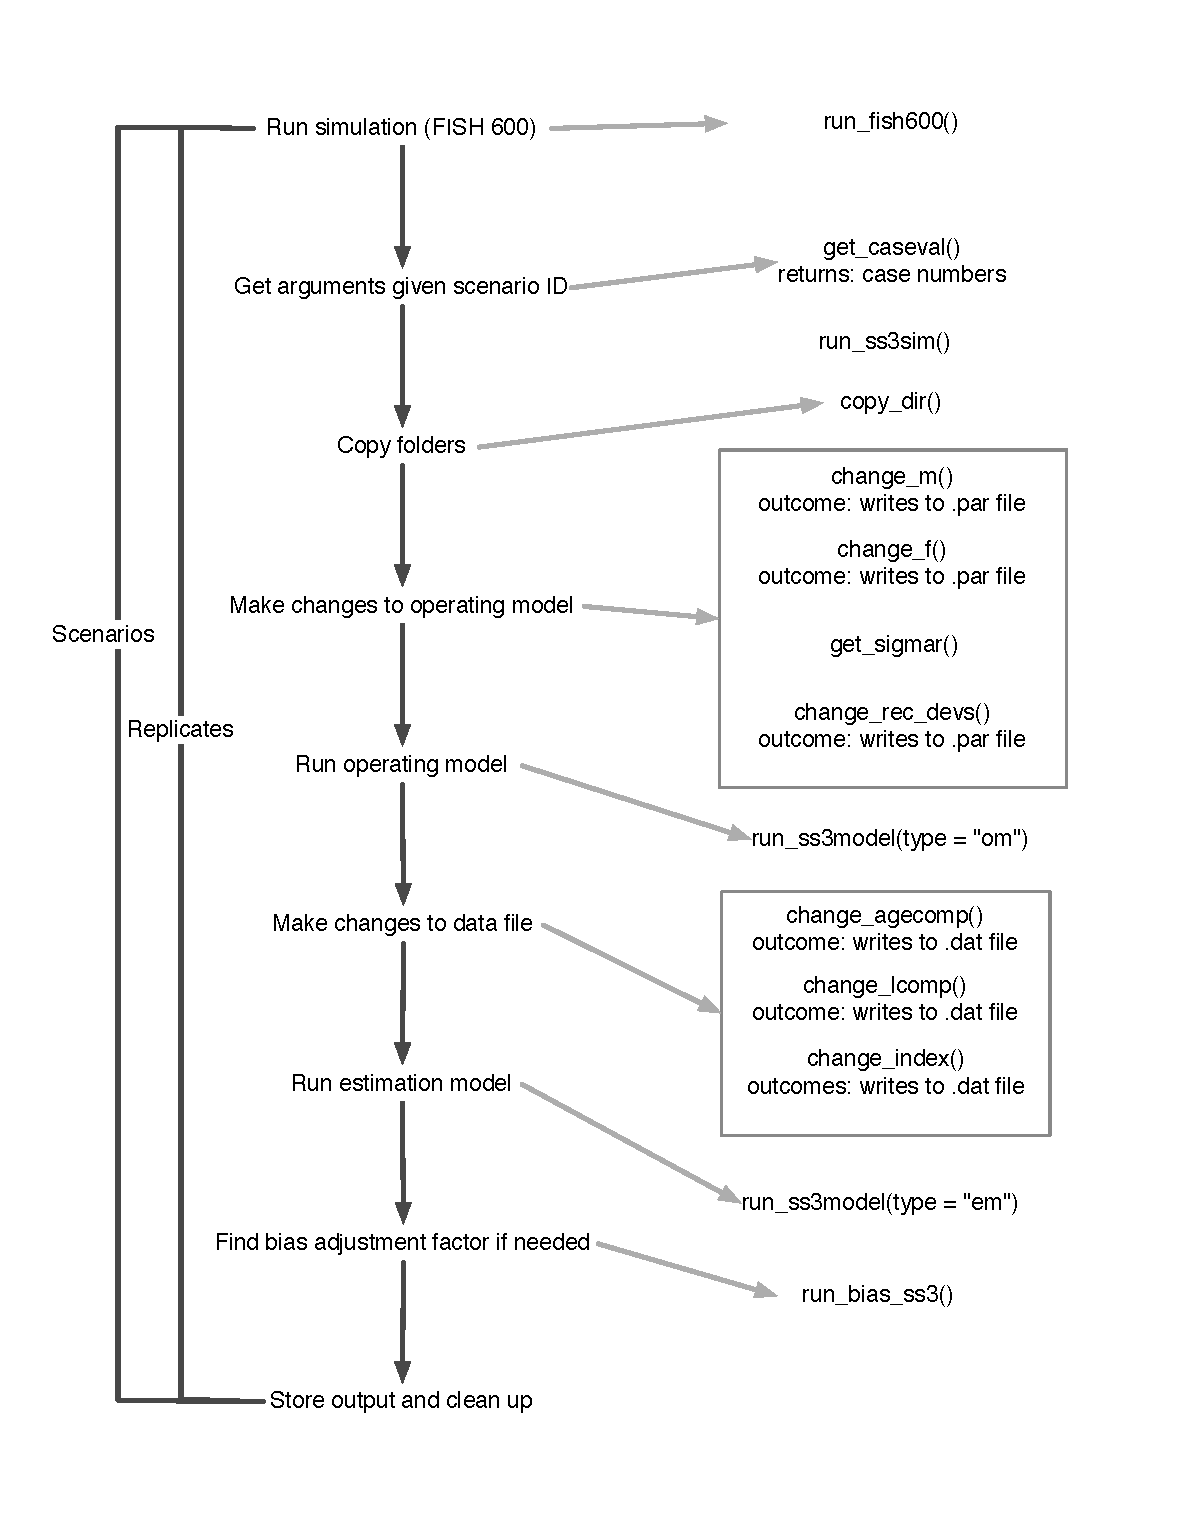
\includegraphics[width=5.5in]{sim-steps.pdf}
  \caption{Simulation steps}
  \label{fig:sim-steps}
\end{figure}


%\noindent
%These functions are used internally by \texttt{run\_simulations} between running
%the operating and estimation models:

%\begin{description}
  %\item[\texttt{change\_lcomp}] Takes a \texttt{data.SS\_new} file, resamples
    %the length compositions from the expected values, and returns a new file
    %with the new length comp samples. Samples can have dimensions, bins, sample
    %sizes, and distributions which are different than those coming from SS.

  %\item[\texttt{change\_agecomp}] Similar to \texttt{change\_lcomp}
    %but for age composition data.

  %\item[\texttt{jitter\_index}] This function is used to create an index of
    %abundance sampled from the expected available biomass for each fleet: survey
    %1 and survey 2 (which mimics the fishery) and add some lognormal errors
    %around it. 
%\end{description}



%\bibliography{/Users/seananderson/Dropbox/tex/jshort,/Users/seananderson/Dropbox/tex/ref}
\end{document}


